\documentclass{standalone}

%----------------------------------------------------------------------------------------------%
%                                 Packages and basic declarations
%----------------------------------------------------------------------------------------------%

\usepackage[utf8]{inputenc}
\usepackage{pgfplots}
\usepackage{tikz}


%----------------------------------------------------------------------------------------------%
%----------------------------------------------------------------------------------------------%
%                                            DOCUMENT STARTS
%----------------------------------------------------------------------------------------------%
%----------------------------------------------------------------------------------------------%

\begin{document}


%Tikz picture starts%

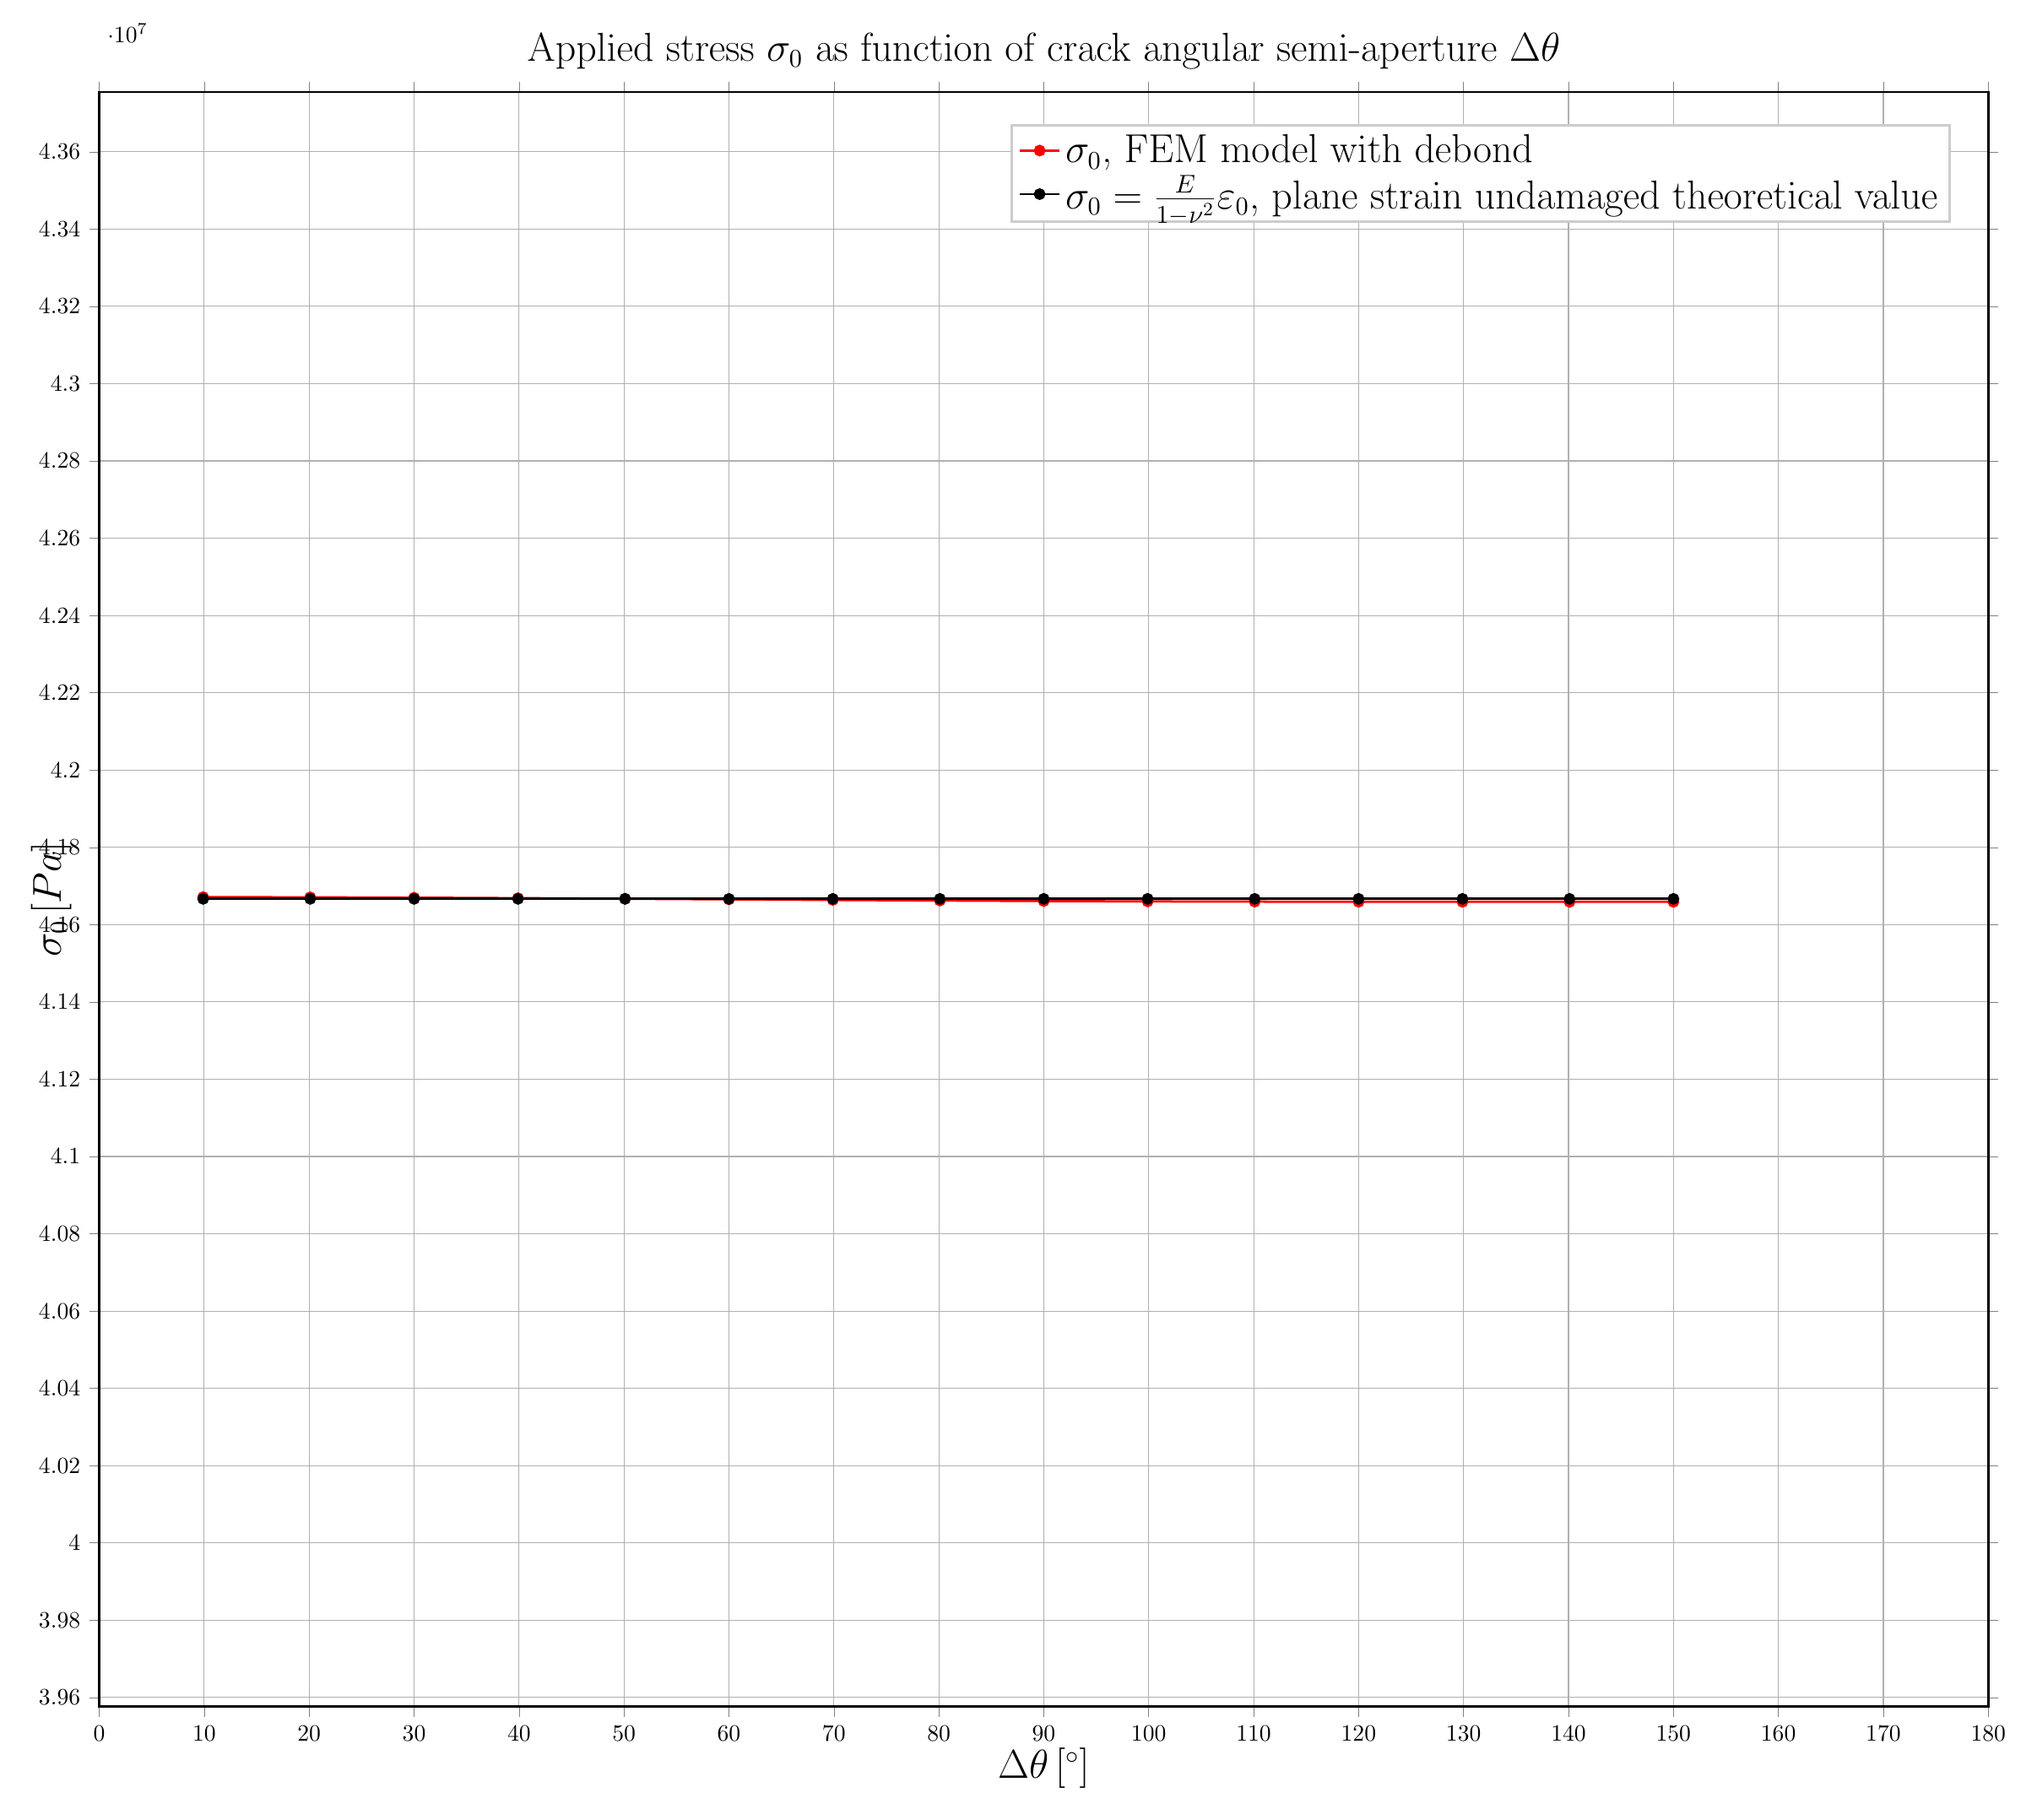
\begin{tikzpicture}

%Tikz axis starts%

\begin{axis}[width=30cm,
title={Applied stress $\sigma_{0}$ as function of crack angular semi-aperture  $\Delta\theta$},
title style={font=\fontsize{16}{8}\selectfont},
xlabel style={at={(axis description cs:0.5,-0.02)},anchor=north,font=\fontsize{16}{8}\selectfont},
ylabel style={at={(axis description cs:-0.01,.5)},anchor=south,font=\fontsize{16}{8}\selectfont},
xlabel={$\Delta\theta\left[^{\circ}\right]$},ylabel={$\sigma_{0}\left[Pa\right]$},
xmin=0.0,
xmax=180.0,
ymin=39575953.6737,
ymax=43754829.5309,
tick align=outside,
tick label style={font=\normalsize},
xtick={0.0,10.0,20.0,30.0,40.0,50.0,60.0,70.0,80.0,90.0,100.0,110.0,120.0,130.0,140.0,150.0,160.0,170.0,180.0},
xmajorgrids,
x grid style={lightgray!92.026143790849673!black},
ymajorgrids,
y grid style={lightgray!92.026143790849673!black},
line width=0.35mm,
legend style={draw=white!80.0!black,font=\fontsize{16}{12}\selectfont},
legend entries={{$\sigma_{0}$, FEM model with debond},{$\sigma_{0}=\frac{E}{1-\nu^{2}}\varepsilon_{0}$, plane strain undamaged theoretical value}},
legend cell align={left}
]

\addplot[red,smooth,mark=*]
table{
9.90004415946 41671266.2199
20.1000992556 41670644.8552
29.9998676461 41669686.9606
39.8998375273 41668449.0787
50.1001615621 41666969.7302
60.0001314432 41665431.4314
69.8999032489 41663883.0065
80.0999574912 41662376.3595
90.0000025045 41661113.7897
99.9000475177 41660139.895
110.10010176 41659470.8845
119.999866736 41659111.7517
129.899843447 41658956.7432
140.100157236 41658913.9197
150.000133948 41658910.5739
};

\addplot[black,smooth,mark=*]
table{
9.90004415946 41666666.6667
20.1000992556 41666666.6667
29.9998676461 41666666.6667
39.8998375273 41666666.6667
50.1001615621 41666666.6667
60.0001314432 41666666.6667
69.8999032489 41666666.6667
80.0999574912 41666666.6667
90.0000025045 41666666.6667
99.9000475177 41666666.6667
110.10010176 41666666.6667
119.999866736 41666666.6667
129.899843447 41666666.6667
140.100157236 41666666.6667
150.000133948 41666666.6667
};

\end{axis}
%Tikz axis ends%


\end{tikzpicture}
%Tikz picture ends%


\end{document}

%----------------------------------------------------------------------------------------------%
%----------------------------------------------------------------------------------------------%
%                                            DOCUMENT ENDS
%----------------------------------------------------------------------------------------------%
%----------------------------------------------------------------------------------------------%

